\section{Discussion and Analysis}
\label{sec:discussion}

In this section we discuss our results and compare them to the human score. We elaborate on potential limiting factors, which may be capping the maximum achievable accuracy. Furthermore, we analyze the model internals, try to interpret them, and distinguish between hard and easy samples in the dataset.

\subsection{Accuracy}

The page rank estimation task is difficult. Our model is provided with screenshots of up to eight webpages of a domain as well as their link structure. Given two samples of that kind, guessing the relative ranking is hard. In the real world, a website's popularity depends on many factors other than its look. By achieving accuracies significantly beyond random guessing (50\%), we do however show that a website's look correlates to some extent with its rank. Obviously, a deduction on the causal relationship between look and rank (or the other way around?) would be purely speculative.

The human score gives an idea of the performance of our model. Even though the model achieves super-human results, it seems unlikely that more sophisticated methods can push the accuracy much further to, say, 90\%. We suspect the upper limit of purely vision-based rank estimation to be below 70\%.

Another aspect of difficulty is noise in the dataset: When crawling and screenshotting 100k websites, some errors are almost inevitable. A small but not negligible percentage of our data is therefore corrupt, e.g. because the website has not finished loading by the time we took the screenshot. Consequently, our model is confronted with all- or almost all-black screenshots occasionally, which harms the training process.

It is noteworthy that the dataset size was sufficient to prevent our CNN architecture from overfitting. We saw no need to make use of regularization methods such as weight decay or data augmentation because the accuracy on training and validation data was almost the same throughout all training runs. We therefore suspect that a model with greater capacity might be able to capture more fine-grained details of screenshots, thereby achieving a higher accuracy.

The accuracy score as proposed in Equation~\ref{eq:acc} has some \textit{unfairness} to it, because the distance of two compared samples is disregarded. For example, a erroneous assessment of the relative ranking of two samples with ranks \#12,000 and \#12,001 is contributing to the accuracy just like the confusion of samples with ranks \#1,000 and \#25,000, even though the latter should presumably be easier to disentangle. Figure~\ref{fig:accvsrank} supports this hypothesis by plotting the mean accuracy against the sample rank. Samples at the end of the spectrum tend to have considerably higher accuracy scores than the ones in the middle, because on average they are juxtaposed to samples with a rank further away from them than samples in the middle. Note that an improvement from 58\% to 64\% is an improvement by a factor of two, because random guessing is at 50\%.
Alternative accuracy metric formulations could take the difficulty of a pairwise comparison into account.

\begin{figure}
    \centering
    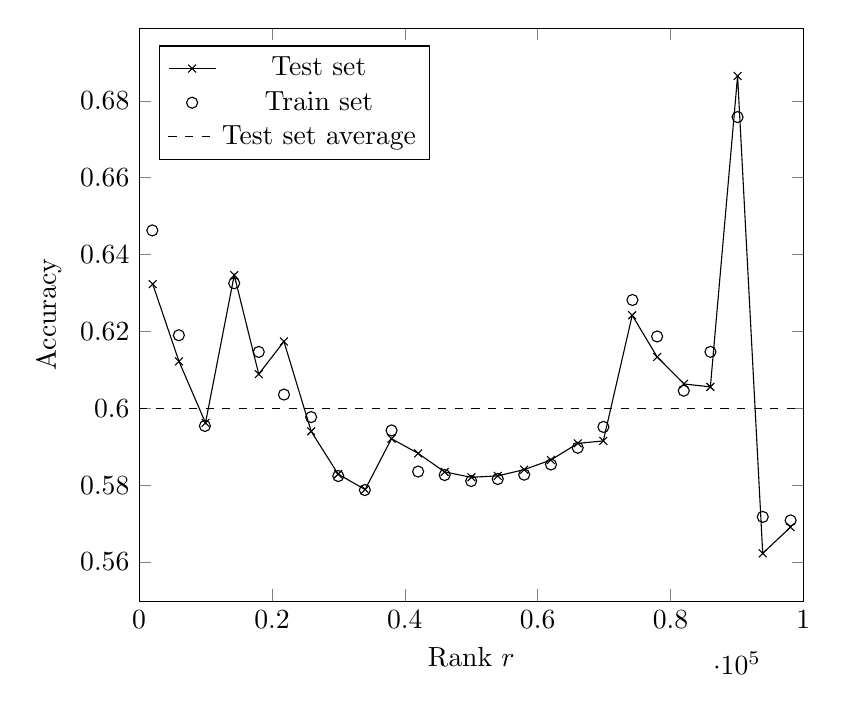
\begin{tikzpicture}

        \pgfplotsset{
            scale only axis,
        }
      
        \begin{axis}[
          legend pos=north west,
          xlabel=Rank $r$,
          ylabel=Accuracy,
          xmin=1,xmax=100000,
        ]
          %\addplot[mark=x,color=black,error bars/.cd, y dir=both,y explicit]
          \addplot[mark=x,color=black]
       coordinates { 
      (2042.0927536231884, 0.6323095560073853) +- (0.252880334854126,0.252880334854126)
      (5994.739130434783, 0.6122098565101624) +- (0.23341456055641174,0.23341456055641174)
      (9987.672131147541, 0.5961850881576538) +- (0.22007544338703156,0.22007544338703156)
      (14314.282571912014, 0.6346387267112732) +- (0.19101302325725555,0.19101302325725555)
      (18001.915745856353, 0.6088740229606628) +- (0.16929037868976593,0.16929037868976593)
      (21796.904761904763, 0.6173704266548157) +- (0.152631938457489,0.152631938457489)
      (25896.116013071896, 0.5939950942993164) +- (0.14189182221889496,0.14189182221889496)
      (29956.708053691276, 0.5828483700752258) +- (0.12687844038009644,0.12687844038009644)
      (34018.020188425304, 0.5788435935974121) +- (0.10543978214263916,0.10543978214263916)
      (37994.73270013568, 0.592072069644928) +- (0.07398778200149536,0.07398778200149536)
      (42004.752380952385, 0.5882502198219299) +- (0.05585600063204765,0.05585600063204765)
      (45999.76454668471, 0.5834199786186218) +- (0.042080748826265335,0.042080748826265335)
      (50028.14344827586, 0.5820223093032837) +- (0.03431824594736099,0.03431824594736099)
      (53989.265027322406, 0.5824041962623596) +- (0.04247155413031578,0.04247155413031578)
      (57966.04674220963, 0.5840225219726562) +- (0.05858512595295906,0.05858512595295906)
      (61993.13711911358, 0.586538553237915) +- (0.07541247457265854,0.07541247457265854)
      (66035.42020497804, 0.590856671333313) +- (0.0997852087020874,0.0997852087020874)
      (69878.57388316152, 0.5914943218231201) +- (0.11854474246501923,0.11854474246501923)
      (74233.90106007067, 0.6241846680641174) +- (0.1272871345281601,0.1272871345281601)
      (77989.69867060562, 0.6133634448051453) +- (0.1402067393064499,0.1402067393064499)
      (82030.64427480916, 0.6063210964202881) +- (0.17285984754562378,0.17285984754562378)
      (86000.5987933635, 0.6055595278739929) +- (0.20112822949886322,0.20112822949886322)
      (90098.17037037037, 0.686475932598114) +- (0.19338952004909515,0.19338952004909515)
      (93881.48888888888, 0.5622369647026062) +- (0.2505538761615753,0.2505538761615753)
      (98061.09816971714, 0.569052517414093) +- (0.26824629306793213,0.26824629306793213)
      };\label{test_set}
      
          \addplot[only marks,mark=o,color=black]
            coordinates{
      (1982.0199443413728, 0.6462764739990234) +- (0.2512509226799011,0.2512509226799011)
      (5978.758321933425, 0.6189908385276794) +- (0.2340804934501648,0.2340804934501648)
      (9902.487074030552, 0.5953881144523621) +- (0.22232778370380402,0.22232778370380402)
      (14307.361990950227, 0.6325339078903198) +- (0.19089166820049286,0.19089166820049286)
      (18004.98867240598, 0.6146559119224548) +- (0.17392544448375702,0.17392544448375702)
      (21806.290449438202, 0.603556752204895) +- (0.15489085018634796,0.15489085018634796)
      (25894.420545746387, 0.5976948142051697) +- (0.1361941397190094,0.1361941397190094)
      (29980.35864022663, 0.5823514461517334) +- (0.12486264109611511,0.12486264109611511)
      (33985.87261146497, 0.578705906867981) +- (0.10141576081514359,0.10141576081514359)
      (38000.94506476106, 0.5942217111587524) +- (0.06816687434911728,0.06816687434911728)
      (41999.57528089888, 0.5835291147232056) +- (0.055270206183195114,0.055270206183195114)
      (45996.97393689986, 0.5826137065887451) +- (0.0386173278093338,0.0386173278093338)
      (49984.56206737425, 0.5810558199882507) +- (0.03277594968676567,0.03277594968676567)
      (53996.78541569902, 0.5815796256065369) +- (0.040436532348394394,0.040436532348394394)
      (57971.61578449905, 0.5827121138572693) +- (0.05864390358328819,0.05864390358328819)
      (62001.87233054782, 0.5853626132011414) +- (0.07834165543317795,0.07834165543317795)
      (66026.0411736867, 0.589715838432312) +- (0.10076970607042313,0.10076970607042313)
      (69899.80461711712, 0.5951372981071472) +- (0.11936279386281967,0.11936279386281967)
      (74265.74804570054, 0.6281706094741821) +- (0.12839582562446594,0.12839582562446594)
      (77984.103948026, 0.6186800599098206) +- (0.1424257755279541,0.1424257755279541)
      (81995.44253770151, 0.6045624017715454) +- (0.17524945735931396,0.17524945735931396)
      (86010.70334685598, 0.6146765351295471) +- (0.1952735334634781,0.1952735334634781)
      (90092.59086444008, 0.6757708787918091) +- (0.20028313994407654,0.20028313994407654)
      (93889.90120620333, 0.5717195272445679) +- (0.2455245852470398,0.2455245852470398)
      (98082.11754874652, 0.5708103179931641) +- (0.26858896017074585,0.26858896017074585)
            }; \label{train_set}
          
          \addplot[dashed][domain=1:100000]{0.6};\label{test_set_avg}
          
          \addlegendimage{/pgfplots/refstyle=test_set}\addlegendentry{Test set}
          \addlegendimage{/pgfplots/refstyle=train_set}\addlegendentry{Train set}
          \addlegendimage{/pgfplots/refstyle=test_set_avg}\addlegendentry{Test set average}
        \end{axis}
      
      \end{tikzpicture}
    \caption[Accuracy vs. rank]{Mean accuracy of samples within a certain rank rages. To compute the data points, batches of samples of 4k ranks were grouped and the mean accuracy was computed. There is a clear tendency of samples in the middle to be harder to classify than samples on the extreme ends of the rank spectrum. The model used to create the plot is [baseline+avg], its performance on the entire test set is indicated by the dashed line. The train set points tends to behave similarly as the test set points. At low ranks, the model is significantly better on the training data which may be attributed to the rank dependent weighting function (see Section~\ref{sec:loss}).}
    \label{fig:accvsrank}
\end{figure}

In summary, we can strongly assume that a correlation between page rank and visual features exists. Our model was able to learn these features and make use of them to solve the pairwise ranking task with an accuracy of xx.x\%. Based on the assumption that an upper limit below 70\% exists, which cannot be exceeded by purely vision-based models, the outcomes of our trainings are a success.

\subsection{Model Understanding}

Besides ranking websites our model has the practical purpose of yielding somewhat interpretable information. In this section we try to understand the model internals and its behavior, and deduce information therefrom.

While it is a common method to look at the kernels of CNNs (see e.g. Figure 3 in \cite{krizhevsky:imagenet}), this approach is not reasonably applicable to our architecture because our filter tensors have a spatial dimension of at most $3\times3$. Instead, we analyze the CNN feature maps, retrieve hard and easy samples, and compute the gradient of the output with respect to the input.

\textbf{Activation maps} are internal representations (latent variables) of an input at intermediate stages of a deep model. Specifically, we consider the input as such, and activations of the CNN blocks Block1, Block2, Block3, and Block4 (before pooling and application of the ReLU function). The sizes of these tensors are listed in Table~\ref{tab:activationmaptensors}.

A qualitative analysis of the activation maps suggests that the model learns to discriminate different elements of webpages such as natural images or text. We have observed some filters to get excited by layout elements such as edges and corners. Figure~\ref{fig:activationmaps} shows some cherry-picked filters from all layers.

\begin{table}
    \centering
    \begin{tabular}{lrr}
        \textbf{Activation map} & \textbf{Spatial size (desktop, mobile)} & \textbf{Depth}\\\hline
        \textbf{Input} & $480\times270\mid480\times270$ & $3$\\
        \textbf{Block1} & $480\times270$ & $3$\\
        \textbf{Block2} & $480\times270$ & $3$\\
        \textbf{Block3} & $480\times270$ & $3$\\
        \textbf{Block4} & $480\times270$ & $3$\\
    \end{tabular}
    \caption[Comparison of GN variants]{Comparison of GN variants + to be updated}
    \label{tab:activationmaptensors}
\end{table}

\begin{figure}
    \centering
    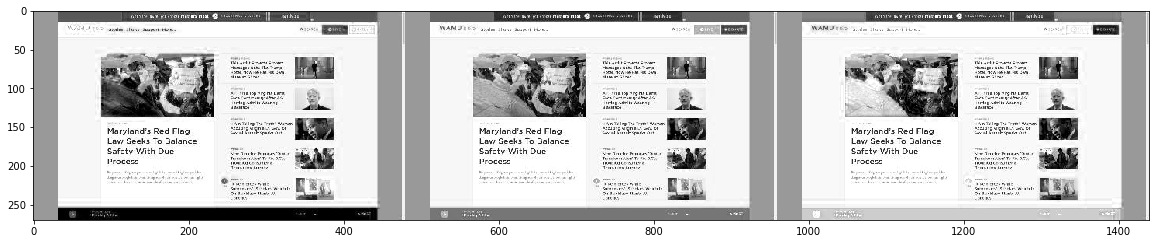
\includegraphics[clip,width=\columnwidth]{resources/analysis/feat-map-0.png}\\
    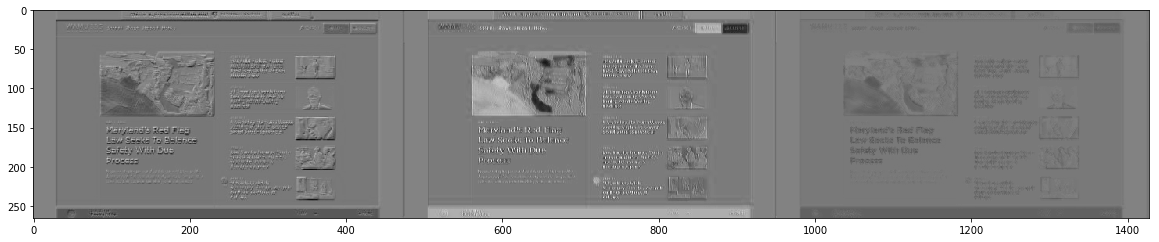
\includegraphics[clip,width=\columnwidth]{resources/analysis/feat-map-1.png}\\
    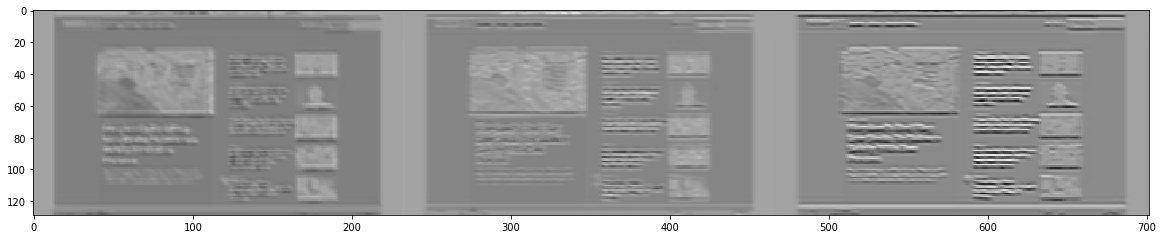
\includegraphics[clip,width=\columnwidth]{resources/analysis/feat-map-2.png}\\
    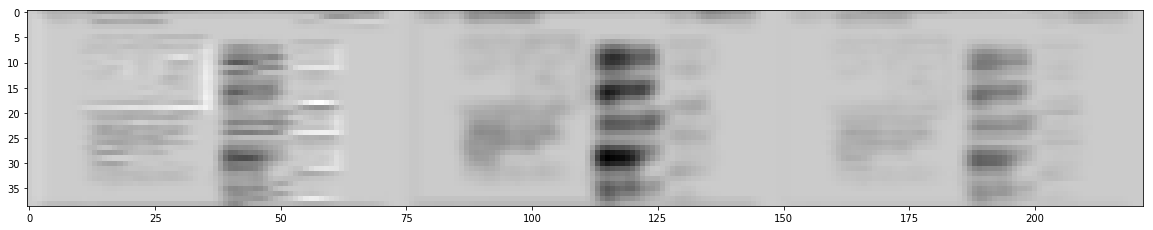
\includegraphics[clip,width=\columnwidth]{resources/analysis/feat-map-3.png}\\
    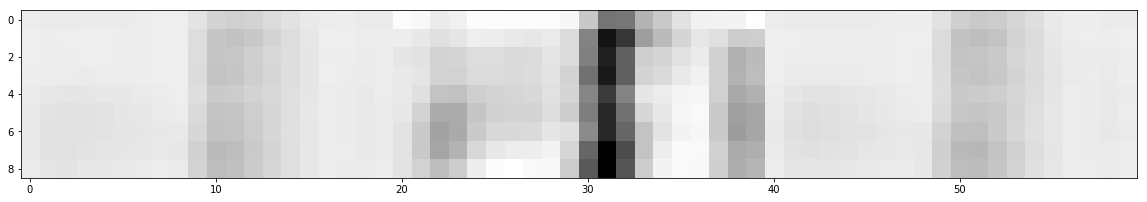
\includegraphics[clip,width=\columnwidth]{resources/analysis/feat-map-4.png}\\
    \caption[Activation maps of the CNN]{Activation maps of the CNN. Top to bottom: Input, Block1, Block2, Block3, and Block4. + This figure will be updated and the caption will describe it.}
    \label{fig:activationmaps}
\end{figure}

We introduce the notion of \textbf{hard and easy samples}. A hard sample from the dataset is characterized by the property that a given model's estimation of its rank diverges significantly from its actual rank. This can be quantized by evaluating Equation~\ref{eq:inference} (inference) and comparing the inferred rank with the ground-truth rank. Samples for which the difference is large are considered hard, because the model has trouble estimating their rank properly. Easy samples are the opposite: Relative to the other samples in the dataset, the model is capable of predicting the correct ranking relatively often.

Hard and easy samples have qualitative meaning because they are representative for websites of their particular rank: Give for instance an easy sample with a high rank, it can be assumed that this sample is representative for high ranked websites. A hard sample with a high rank might have attained its rank for reasons other than its look. On the other hand, easy samples with low rank are representative for websites with a low rank. By comparing easy samples with high/low rank we can distill the visual difference between high and low ranked websites. Note that this is more sophisticated than looking only at the pure dataset, i.e. comparing high-ranked samples with low-ranked samples, because the model acts as a filter, extracting the visually representative samples.

We split the test dataset ranks into 25 bins (each containing 4k samples) and search for the hardest and easiest sample in each of those bins. The first desktop screenshot of each of those samples is depicted in Figure~\ref{fig:hardandeasysamples} (50 screenshots in total). We have noticed that samples in the middle of the spectrum had accuracies much closer to 50\%. For instance, the easiest sample in the bin $r^{(i)}\in{\left\{44000, \dots, 47999\right\}}$ (which is $i=44064$) has an accuracy of just $62.83\%$. All maximum/mininum accuracies vs. ranks can be seen in Figure~\ref{fig:minmaxaccvsrank}.

%\begin{figure}
%    \floatbox[{\capbeside\thisfloatsetup{capbesideposition={left,top},capbesidewidth=4cm}}]{figure}[\FBwidth]
%    {\caption[Easy and hard samples across all ranks]{Easy (left) and hard (right) samples across all ranks from high (top) to low (bottom); best seen on a computer screen. The images are the hardest/easiest samples in rank-bins of size $4000$. Each image corresponds to one cross-mark in Figure~\ref{fig:minmaxaccvsrank}.}\label{fig:hardandeasysamples}}
%    {
\includegraphics[height=\textheight]{resources/hard-easy.jpg}}
%\end{figure}

\begin{figure}
    \centering
    \begin{tikzpicture}

        \pgfplotsset{
        scale only axis,
        }

        \begin{axis}[legend style={at={(0.5,+1.1)},anchor=south},
            xlabel=Rank $r$,
            ylabel=Accuracy,
            xmin=1,xmax=100000,
            ]
            \addplot[name path=F,mark=x,color=black]
            coordinates {
            (55, 0.9988577)
            (4058, 0.95130163)
            (8020, 0.91372573)
            (12572, 0.8788553)
            (16364, 0.84158)
            (20383, 0.796549)
            (24407, 0.76179886)
            (28073, 0.7308363)
            (32071, 0.7000541)
            (36001, 0.6655444)
            (40071, 0.6422774)
            (44064, 0.6283292)
            (51649, 0.6214754)
            (55605, 0.62760776)
            (59829, 0.64065415)
            (63952, 0.66452235)
            (67973, 0.700475)
            (71939, 0.7335417)
            (75917, 0.7663681)
            (79826, 0.80586785)
            (83884, 0.84512717)
            (87970, 0.8857091)
            (90855, 0.9140263)
            (95235, 0.95502913)
            (99609, 0.9919437)
            };\label{max_acc}

            \addplot[name path=G,mark=x,color=black]
            coordinates{
            (450, 0.009799795)
            (4880, 0.061504237)
            (9957, 0.10467143)
            (12899, 0.13112487)
            (16956, 0.17519389)
            (20828, 0.21535502)
            (24155, 0.24685866)
            (28599, 0.2820297)
            (32801, 0.32110864)
            (36635, 0.3725125)
            (40459, 0.40996814)
            (44435, 0.44928756)
            (51995, 0.47556064)
            (55450, 0.4379246)
            (59871, 0.38784343)
            (62559, 0.35898516)
            (67819, 0.3109481)
            (70262, 0.28449467)
            (75932, 0.25335178)
            (79033, 0.20543498)
            (83407, 0.16286899)
            (86852, 0.12360969)
            (91299, 0.09427042)
            (95411, 0.0490591)
            (99866, 0.008537245)
            }; \label{min_acc}

            \addplot[pattern=north west lines, pattern color=brown!50]fill between[of=F and G, soft clip={domain=1:100000}];\label{area}

            \addplot[dashed][domain=1:100000]{0.6};\label{test_set_avg2}
            \addplot[][domain=1:100000]{1-1/100000*x};
            \addplot[solid][domain=1:100000]{0+1/100000*x};\label{test_set_trivial_bound}

            \addlegendimage{/pgfplots/refstyle=max_acc}\addlegendentry{Maximum (easy samples)}
            \addlegendimage{/pgfplots/refstyle=min_acc}\addlegendentry{Minimum (hard samples)}
            \addlegendimage{/pgfplots/refstyle=area}\addlegendentry{All accuracies}
            \addlegendimage{/pgfplots/refstyle=test_set_avg2}\addlegendentry{Average}
            \addlegendimage{/pgfplots/refstyle=test_set_trivial_bound}\addlegendentry{Trivial bound}
        \end{axis}

    \end{tikzpicture}
    \caption[Min/max accuracy vs. rank]{Min/max accuracy of samples in bins of size $4000$ vs. their rank. It is apparent that the model struggles at estimating the rank of samples in the middle correctly, because it is harder. Take for instance the sample with the highest rank: The model could theoretically easily achieve 100\% accuracy by predicting a high value for it. Likewise, it can constantly predict a low value for it, making it a hard sample (accuracy 0\%). This \textit{trivial} predicting gets harder as the ranks diverge from the ends of the spectrum. The solid lines indicate where the trivial bound lies; for a randomly initialized model maximum and minimum would (in the expected value) lay on the trivial bound. Crosses exceeding the solid lines (i.e. crosses above or below the surface enclosed by them) are better than the trivial guessing. It is important to note though, that the samples are drawn from the test set, so the model has not seen them before. The horizontal, dashed line marks the average model performance on the test set.}
    \label{fig:minmaxaccvsrank}
\end{figure}

Our last model analysis method is the computation of the \textbf{gradient $\tensorsym{G}$ of the model output with respect to the input}. It highlights areas, which when changed, have strong influence on the assessment of the given sample. The mathematical formulation is\begin{equation}
    \tensorsym{G}=\frac{\partial f\left(\tensorsym{I}\right)}{\partial\tensorsym{I}}\,,
\end{equation}where $\tensorsym{I}$ can be either a desktop or a mobile image. In the following, the function $f$ is a screenshot feature extractor without graph network. To ensure the gradient is meaningful, we chose only samples which the model classifies with high accuracy, i.e. easy ones.

Figure~\ref{fig:gradwrtinput} shows $\tensorsym{G}$ for an easy sample. Interpretation xxx.

\begin{figure}
    \centering
    % include graphics
    \caption[Areas with high influence on the model prediction]{Areas with high influence on the model prediction, xxx...}
    \label{fig:gradwrtinput}
\end{figure}
